% BabyLM 2026 workshop submission — EMNLP 2026 workshop (ACL) style.
% Build: tectonic main.tex   (or pdflatex + bibtex twice)
\documentclass[11pt]{article}
\usepackage[preprint]{acl}
\usepackage{times}
\usepackage{latexsym}
\usepackage[T1]{fontenc}
\usepackage{microtype}
\usepackage{inconsolata}
\usepackage{graphicx}
\usepackage{booktabs}
\usepackage{amsmath}

% float-only pages (the appendix provenance table) anchor to the top instead
% of centering vertically
\makeatletter
\setlength{\@fptop}{0pt}
\setlength{\@dblfptop}{0pt}
\makeatother

\title{When Does Depth Recursion Pay? A Parameter-Matched Study of\\Weight-Tied Hybrid Transformers on 100M Unique Words}

\author{Aditya Sasidhar \\
  \texttt{telikicherlaadityasasidhar@gmail.com}}

\begin{document}
\maketitle

\begin{abstract}
Weight-tied depth recursion trades computation for effective depth without adding learned parameters. We pre-train five hybrid Gated DeltaNet (GDN) + grouped-query attention (GQA) transformers from scratch on the BabyLM 2026 Strict corpus under one tokenizer, data order, optimizer, and 500M-token budget. Two parameter-matched pairs share their learned parameter tensors and layer inventories; the recursive configuration re-applies each super-block three times and uses effective-depth residual scaling. At the final checkpoint, recursion improves validation loss by 0.026 and 0.019 nats, with the advantage present in nearly every aligned evaluation window. Mean zero-shot BLiMP rises by 3.31 and 4.21 points; the 3:1 gain is consistent across paradigms, whereas the 2:1 mean is driven by heterogeneous, right-tailed effects rather than a broad directional shift. Both recursive models trail their twins at 100M tokens and lead at 200M; the checkpoint spacing cannot determine whether this crossover precedes the epoch boundary or whether repetition causes it. Across architectures, rankings reverse: the recursive hybrids rank first and second on validation loss, while the larger pure-GQA baseline leads BLiMP at 71.07. The controlled evidence therefore supports recursion as a weight-parameter-efficiency mechanism inside these hybrids, not as a compute- or inference-efficiency result; all models have only one training seed.
\end{abstract}

\section{Introduction}
\label{sec:intro}

The BabyLM challenge fixes the training data --- roughly the number of words a human encounters during development --- and asks what modeling choices make the most of it \citep{babylm2026cfp}. Most entries respond with data curricula or training objectives. We instead use the fixed-data setting for what it does best: making an \emph{architectural} question unusually clean to answer.

\begin{quote}
\textbf{If parameters are scarce, is it better to spend them on independent layers, or to re-apply a smaller stack of layers several times with tied weights?}
\end{quote}

Weight-tied depth recursion --- applying the same block of layers repeatedly --- decouples a model's \emph{effective depth} from its parameter count. The idea is old \citep{dehghani2019universal,lan2020albert} and now spans from-scratch small models \citep{liu2024mobilellm}, large recurrent-depth pre-training \citep{geiping2025recurrent}, conversion of pre-trained models \citep{bae2024relaxed}, and adaptive recursion \citep{bae2025mor}. We ask a narrower controlled question not answered by those studies: under a small-data budget, what changes when a modern hybrid re-applies a fixed inventory of learned layers rather than applying it once?

We run it inside a modern \emph{hybrid} architecture that interleaves Gated DeltaNet linear-attention layers \citep{yang2025gateddeltanet} with softmax grouped-query attention layers \citep{ainslie2023gqa} in fixed ratios, following the design popularized by Qwen3-Next \citep{qwen2025next}. Hybrids are a natural host for the question: a hybrid \emph{ratio unit} (e.g., GDN--GDN--GQA) is a self-contained token-mixing block, so recursion has an obvious granularity --- repeat the unit. They also let us test a second, related hypothesis: that small models are constrained by the \emph{density of softmax attention} --- the intuition that precise, unbounded-memory retrieval is what a small budget can least afford to cut.

\paragraph{Contributions.}
\begin{enumerate}
  \item \textbf{A matched recursion comparison.} Two pairs have identical learned layer inventories and parameter counts (46{,}913{,}888 and 63{,}487{,}504 non-embedding parameters), with one training stream and recipe. The recursive configuration differs through tied re-application and effective-depth residual scaling.
  \item \textbf{Evaluation with paired uncertainty.} Both loss gains are consistent across aligned windows, and the 3:1 BLiMP gain is consistent across paradigms. The positive 2:1 BLiMP mean is not a broad directional shift; bootstrap intervals and exact sign tests expose this distinction, while the single-seed limitation remains explicit.
  \item \textbf{A scoped architectural result.} Loss and grammatical rankings reverse across architectures; attention density is confounded, and position-wise gains are broad with only modest late widening. The evidence supports a within-pair weight-efficiency claim, not compute efficiency or a causal long-range mechanism.
\end{enumerate}

\paragraph{Evaluation note.} A training-time logger averaged per-batch means and biased some losses by $-0.025$. All paper numbers are recomputed from checkpoints with uniform weighting; Appendix~\ref{app:repro} documents the pitfall.

\paragraph{Code and artifacts.} Source code, evaluation artifacts, and reproduction scripts are available at \url{https://github.com/adityasasidhar/recursive-babylm}.

\section{Related Work}
\label{sec:related}

\paragraph{Parameter sharing across depth.} Universal Transformers \citep{dehghani2019universal} apply one block recurrently with adaptive halting; ALBERT \citep{lan2020albert} ties encoder layers. Most directly, MobileLLM-LS pre-trains 125M- and 350M-parameter decoder-only models with immediate block-wise sharing and reports downstream gains \citep{liu2024mobilellm}. \citet{geiping2025recurrent} scale a recurrent-depth decoder to 3.5B parameters and 800B tokens with variable test-time recurrence. Relaxed Recursive Transformers convert pre-trained models and soften ties with layer-wise LoRA \citep{bae2024relaxed}, while Mixture-of-Recursions learns token-specific depths \citep{bae2025mor}. Our novelty is therefore not from-scratch sharing itself, but two exact learned-parameter-matched comparisons inside a GDN--GQA hybrid under a controlled small-data stream.

\paragraph{Linear attention and the delta rule.} DeltaNet-style linear attention maintains a fast-weight state updated by the delta rule and is parallelizable over sequence length \citep{yang2024deltanet}. Gated DeltaNet adds a data-dependent decay gate and improves over Mamba2 and DeltaNet \citep{yang2025gateddeltanet}. We use the reference Triton kernels from the \texttt{flash-linear-attention} library \citep{yang2024fla}.

\paragraph{Hybrid architectures.} A minority of softmax-attention layers interleaved with a majority of linear-attention layers preserves most of full attention's quality at a fraction of its inference cost; Qwen3-Next \citep{qwen2025next} adopts a 3:1 Gated-DeltaNet:attention ratio at 80B scale. We evaluate 2:1 and 3:1 ratios at BabyLM scale and use the ratio unit as the unit of recursion.

\paragraph{Sample-efficient pre-training.} The BabyLM workshop series \citep{warstadt2023findings,babylm2026cfp} fixes the corpus (Strict track: 100M words; repetition allowed up to 1B words of total exposure) so that architectural and algorithmic effects are comparable across submissions. Our runs consume ${\sim}295$M words of exposure each, within the allowed budget.

\section{Models}
\label{sec:models}

All five variants share one spine: a decoder-only pre-norm transformer with $d_{\text{model}} = 768$, RMSNorm \citep[$\epsilon = 10^{-5}$]{zhang2019rmsnorm}, SwiGLU feed-forward blocks \citep{shazeer2020glu} with $d_{\text{ff}} = 2304$ (a fixed $3\times$ multiplier for \emph{all} variants), tied input/output embeddings, and the BabyLM-community BPE tokenizer (vocabulary 16{,}384). Every token-mixing layer is followed by one SwiGLU FFN sub-layer with its own residual connection.

\paragraph{GQA layers} use 12 query heads and 4 KV heads of dimension 64, rotary position embeddings \citep{su2021roformer} with base 10{,}000, and per-head RMS QK-normalization \citep{henry2020qknorm}. Softmax attention runs FlashAttention-3 on Hopper GPUs \citep{shah2024flashattention3} with an SDPA fallback elsewhere.

\paragraph{GDN layers} are Gated DeltaNet layers \citep{yang2025gateddeltanet} as implemented in \texttt{flash-linear-attention} v0.5.1: 12 heads of dimension 64, value expansion 1, output gating and short (size-4) depthwise convolutions enabled, and a delta-rule fast-weight state with data-dependent decay. GDN applies its own L2 normalization to queries and keys.

\subsection{The five variants}
\label{sec:variants}

\begin{table*}[t]
\centering
\small
\setlength{\tabcolsep}{5.5pt}
\begin{tabular}{llccccc}
\toprule
Variant & Attention mix & Unique layers & Super-blocks $\times$ R & Eff.\ depth & Non-emb.\ params & Total params \\
\midrule
GQA baseline  & pure GQA      & 10 & ---          & 10 & 68{,}830{,}208 & 81{,}413{,}120 \\
GDN 2:1       & GDN:GQA = 2:1 & 6  & ---          & 6  & 46{,}913{,}888 & 59{,}496{,}800 \\
GDN 3:1       & GDN:GQA = 3:1 & 8  & ---          & 8  & 63{,}487{,}504 & 76{,}070{,}416 \\
Recursive 2:1 & GDN:GQA = 2:1 & 6  & $2 \times 3$ & 18 & 46{,}913{,}888 & 59{,}496{,}800 \\
Recursive 3:1 & GDN:GQA = 3:1 & 8  & $2 \times 3$ & 24 & 63{,}487{,}504 & 76{,}070{,}416 \\
\bottomrule
\end{tabular}
\caption{The five pre-trained variants. GDN 2:1 / Recursive 2:1 and GDN 3:1 / Recursive 3:1 are exact parameter-matched pairs.}
\label{tab:variants}
\end{table*}

A \emph{ratio unit} is (GDN, GDN, GQA) for 2:1 and (GDN, GDN, GDN, GQA) for 3:1. The non-recursive hybrids stack two units. The recursive hybrids contain \textbf{two independent super-blocks in sequence, each holding one ratio unit, each applied $R = 3$ times with weights tied within that super-block} (never across super-blocks). Unrolled, Recursive 2:1 computes 18 layer applications with the parameters of 6 layers --- and, notably, applies softmax attention 6 times per token where its twin applies it twice.

Within each pair, the models have identical learned layer inventories and parameter counts \emph{to the digit}; the recursive configuration applies the super-blocks three times rather than once and uses the effective-depth initialization below (Table~\ref{tab:variants}). The pure-GQA baseline is a no-GDN reference at its own, larger size; we use it as a size anchor and as the maximum-attention-density point in the descriptive analysis of Section~\ref{sec:density}.

\subsection{Initialization}
\label{sec:init}

Weights are drawn from $\mathcal{N}(0, 0.02^2)$; residual-output projections (attention output, FFN down-projection) are scaled by $1/\sqrt{2 D_{\text{eff}}}$, where $D_{\text{eff}}$ is the \emph{effective} depth --- 18 or 24 for the recursive models, the plain layer count otherwise. This principled depth-aware choice is nevertheless a second within-pair configuration difference. The experiment therefore identifies the recursive configuration (tying plus its depth-aware scaling), not tying alone; an alternative-scaling ablation is needed to separate them.

\section{Experimental Setup}
\label{sec:setup}

\paragraph{Data.} We train on the official BabyLM 2026 Strict corpus (six domain files, ${\sim}100$M words) and validate on the official dev split, excluded from the training bins at preprocessing time.\footnote{\texttt{BabyLM-community/BabyLM-2026-Strict} and \texttt{BabyLM-community/BabyLM-dev} on the HuggingFace Hub.} Under the shared 16{,}384-vocabulary tokenizer, one epoch is 169{,}741{,}563 tokens ($\approx$1.70 tokens per whitespace word).

\paragraph{Recipe (identical for all five runs).} Sequence length 4{,}096; batch 32 sequences = 131{,}072 tokens per optimizer step; 3{,}814 steps = 499{,}908{,}608 tokens $\approx$ 2.9 epochs $\approx$ 295M words of exposure --- compliant with the Strict-track rules ($\leq$100M unique words; $\leq$1B words of total exposure). AdamW \citep{loshchilov2019adamw} with $\beta = (0.9, 0.95)$, weight decay 0.1 on matrices only, gradient clipping at 1.0; peak learning rate $6\times10^{-4}$ with 250 warmup steps and cosine decay to 10\% of peak; bf16 autocast with fp32 master weights; seed 42. Data order is identical across variants by construction: every run draws the same seeded shuffle of 4{,}096-token chunks each epoch, so all five models see exactly the same tokens in exactly the same order.

\paragraph{Evaluation protocol.} All validation numbers are recomputed from retained checkpoints (one per 100M training tokens, plus final) over the same 488 non-overlapping 4{,}096-token windows, with uniform per-token weighting and an identical code path. The 2M-token prefix was fixed to bound the cost of evaluating 25 checkpoints, not selected by model performance. Because preprocessing concatenates sorted domain files, it comprises all 1.738M tokens of BNC Spoken and the first 0.261M tokens of CHILDES rather than a domain-balanced dev sample. Paired uncertainty estimates resample aligned windows; Appendix~\ref{app:repro} documents their scope and the training-logger bug.

\paragraph{Hardware and cost.} Each variant trains on a single H100-80GB (Modal): 18.8--27.6 min for the non-recursive models, 46.2 and 62.1 min for Recursive 2:1 and 3:1 --- about 3 GPU-hours for the grid. Gradient accumulation splits the 32-sequence batch into micro-batches of 16 (8 for Recursive 3:1, whose 24-layer effective depth needs a smaller activation footprint); this leaves the optimizer-step mathematics unchanged.

\section{Results}
\label{sec:results}

Table~\ref{tab:final} reports final validation metrics after the full 500M-token budget; Table~\ref{tab:traj} and Figure~\ref{fig:curves} trace the trajectories; Figure~\ref{fig:scatter} summarizes the parameter--quality trade-off; Table~\ref{tab:pos} breaks the losses down by context position; and Table~\ref{tab:blimp} reports zero-shot BLiMP.

\begin{table*}[t]
\centering
\small
\begin{tabular}{lcccccc}
\toprule
Model & Non-emb.\ params & Eff.\ depth & Val loss $\downarrow$ & Val ppl $\downarrow$ & bpt $\downarrow$ & Train loss \\
\midrule
\textbf{Recursive 3:1} & 63.5M & 24 & \textbf{3.0926} & \textbf{22.03} & \textbf{4.462} & 2.552 \\
Recursive 2:1          & 46.9M & 18 & 3.1072          & 22.36          & 4.483          & 2.588 \\
GDN 3:1                & 63.5M & 8  & 3.1121          & 22.47          & 4.490          & 2.568 \\
GQA baseline           & 68.8M & 10 & 3.1244          & 22.75          & 4.508          & 2.609 \\
GDN 2:1                & 46.9M & 6  & 3.1333          & 22.95          & 4.520          & 2.614 \\
\bottomrule
\end{tabular}
\caption{Final metrics on the fixed dev slice after 500M training tokens (uniform per-token weighting; single seed). Loss in nats/token; bpt = bits per token. Rows sharing a parameter count are learned-parameter-matched configurations.}
\label{tab:final}
\end{table*}

\begin{table*}[t]
\centering
\small
\begin{tabular}{lccccc}
\toprule
Model & 100M & 200M & 300M & 400M & 500M \\
\midrule
Recursive 2:1 & 3.5121 & 3.2778 & 3.1803 & 3.1315 & 3.1072 \\
GDN 2:1       & 3.5033$^{\dagger}$ & 3.2923 & 3.2033 & 3.1564 & 3.1333 \\
Recursive 3:1 & 3.5292 & \textbf{3.2712} & \textbf{3.1676} & \textbf{3.1174} & \textbf{3.0926} \\
GDN 3:1       & \textbf{3.4952}$^{\dagger}$ & 3.2739 & 3.1803 & 3.1352 & 3.1121 \\
GQA baseline  & 3.5560 & 3.3041 & 3.2052 & 3.1505 & 3.1244 \\
\midrule
\emph{pair $\Delta$ (2:1, gdn $-$ rec)} & $-0.009$ & $+0.014$ & $+0.023$ & $+0.025$ & $+0.026$ \\
\emph{pair $\Delta$ (3:1, gdn $-$ rec)} & $-0.034$ & $+0.003$ & $+0.013$ & $+0.018$ & $+0.019$ \\
\bottomrule
\end{tabular}
\caption{Validation loss (nats) at each retained checkpoint (uniform weighting; one epoch $\approx$169.7M tokens). Bold marks the overall leader at a checkpoint; $\dagger$ marks the within-pair leader at 100M. Both recursive models trail their twins at 100M and lead at 200M, but the grid does not locate the crossover relative to the epoch boundary.}
\label{tab:traj}
\end{table*}

\begin{figure*}[t]
\centering
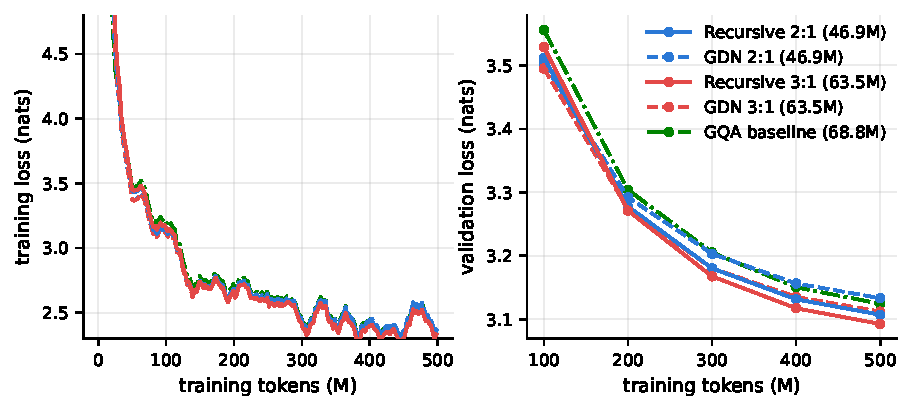
\includegraphics[width=\textwidth]{figures/loss_curves.pdf}
\caption{Training loss (left, smoothed, from training logs) and checkpoint validation loss (right, uniform protocol) versus training tokens. Hue encodes the ablation pair (blue = 2:1, red = 3:1, green = baseline); solid lines are recursive models, dashed are their non-recursive twins. All runs are stable --- zero loss spikes across 19{,}070 optimizer steps in total --- and every model is still improving when the budget ends.}
\label{fig:curves}
\end{figure*}

\begin{figure}[t]
\centering
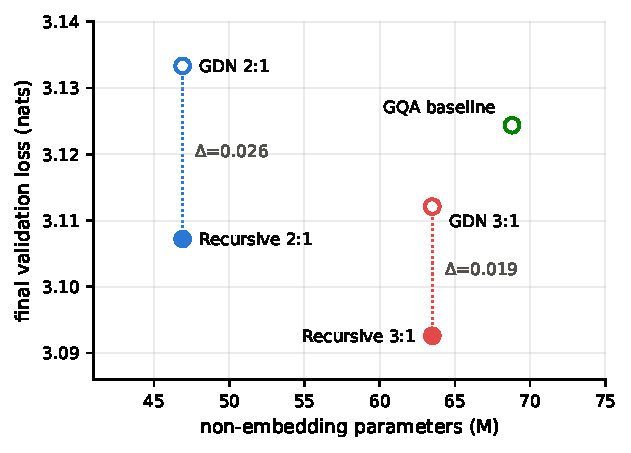
\includegraphics[width=\columnwidth]{figures/params_vs_val.pdf}
\caption{The parameter--quality trade-off. Recursion improves both parameter-matched pairs ($\Delta$ = 0.026 and 0.019 nats), and both recursive models beat every non-recursive model, including the larger pure-attention baseline.}
\label{fig:scatter}
\end{figure}

\paragraph{Recursion improves both matched configurations.} At the final checkpoint, the recursive member lowers validation loss by 0.026 nats (2.6\% perplexity) in the 2:1 pair and 0.019 nats (2.0\%) in the 3:1 pair. A paired 100{,}000-resample bootstrap over the 488 aligned windows gives differences (non-recursive minus recursive) of 0.0261 [0.0248, 0.0274] and 0.0195 [0.0183, 0.0207] nats (95\% percentile intervals). Exact paired sign tests show the same unusually consistent pattern: recursion wins on 480/488 windows in the 2:1 pair ($p=1.92\times10^{-130}$) and 462/488 in the 3:1 pair ($p=2.64\times10^{-104}$). These statistics quantify finite evaluation-sample uncertainty, not training-seed variance, and the domain-contiguous windows are not fully independent. Descriptively, the two recursive models finish first and second among all five.

\paragraph{The advantage appears after 100M tokens.} Each recursive model trails its twin at 100M and leads at 200M; the pair gaps then widen through the retained checkpoints. Because one epoch is 169.7M tokens, this interval straddles the first epoch boundary. The grid cannot determine whether the crossover occurs before or after repeated examples begin, nor distinguish repetition from additional optimization steps. Linear interpolation gives token-efficiency point estimates of 21\% and 16\%, but the 100M checkpoint spacing makes them approximate.

\paragraph{Fitting and generalization now agree.} The recursive member also has the lower \emph{training} loss in both pairs (2.588 vs.\ 2.614; 2.552 vs.\ 2.568): the extra effective depth adds fitting capacity, and under this budget that capacity transfers to held-out data rather than overfitting the (repeated) corpus.

\paragraph{Stability and cost.} All five runs completed with zero loss spikes and gradient norms settling at 0.24--0.26. The recursive models pay for their quality in compute, not parameters: at fixed parameters they execute ${\sim}3\times$ the layer FLOPs per token, and throughput drops accordingly (181k and 134k tokens/s vs.\ 443k and 353k for their twins; Appendix~\ref{app:repro}).

\subsection{Zero-shot grammatical generalization}
\label{sec:blimp}

We evaluate each final checkpoint on the official BabyLM 2026 full BLiMP and BLiMP Supplement sets \citep{warstadt2020blimp}: 59{,}875 and 5{,}218 minimal pairs, respectively. Following the official causal protocol, candidates are ranked by summed log-probability over all non-BOS sentence tokens, and scores are macro-averaged over the 67 BLiMP paradigms (five supplement tasks). Table~\ref{tab:blimp} reports accuracy at temperature 1.

\begin{table}[t]
\centering
\small
\begin{tabular}{lrr}
\toprule
Model & BLiMP $\uparrow$ & Supplement $\uparrow$ \\
\midrule
\textbf{GQA baseline} & \textbf{71.07} & \textbf{59.59} \\
Recursive 3:1         & 67.48 & 55.17 \\
Recursive 2:1         & 65.56 & 53.30 \\
GDN 3:1               & 63.27 & 53.93 \\
GDN 2:1               & 62.24 & 52.28 \\
\midrule
\emph{$\Delta$ 2:1 (rec $-$ gdn)} & $+3.31$ & $+1.01$ \\
\emph{$\Delta$ 3:1 (rec $-$ gdn)} & $+4.21$ & $+1.24$ \\
\bottomrule
\end{tabular}
\caption{Zero-shot grammatical minimal-pair accuracy on the official BabyLM 2026 full evaluation sets. Scores macro-average paradigms/tasks; bold marks the overall leader. Pair deltas are point estimates.}
\label{tab:blimp}
\end{table}

\paragraph{The 3:1 pair provides the clearest evidence beyond LM loss.} Paired bootstrap over the 67 paradigms gives a 3:1 recursion gain of $+4.21$ [2.43, 6.11] points. It wins on 46 paradigms, loses on 20, and ties on one (two-sided exact sign test $p=.0019$), so both the mean and direction of the effect agree. The 2:1 mean gain is $+3.31$ [0.38, 6.85], but it wins on only 37 paradigms and loses on 30 ($p=.464$). Its median gain is just $+0.64$ points: a smaller subset of large positive effects produces a right tail and pulls up the mean, so the bootstrap CI does not establish a broad paradigm-level shift. The tests answer different questions rather than contradicting each other. The five-task supplement is too small for its positive point estimates to be conclusive: $+1.01$ [$-0.79$, 3.49] and $+1.24$ [$-2.81$, 6.13]. All of these statistics quantify evaluation-set sampling only and do not replace independent training seeds.

\paragraph{The across-architecture ranking reverses.} The pure-GQA baseline, fourth on validation loss, ranks first on both grammatical suites (71.07 / 59.59). Recursive 3:1 is the strongest hybrid but does not overtake it. For external scale, the official BabyLM 2026 Strict GPT-2 reference reports 74.53 / 65.00; that model differs in architecture, recipe, and exposure, so this is context rather than a controlled comparison.\footnote{\url{https://github.com/babylm-org/babylm-eval\#strict--strict-small}} Our results are not yet a complete Challenge score (Limitations).

\subsection{Coarse density comparison: no identified causal effect}
\label{sec:density}

A plausible reading of hybrid designs is that softmax attention --- with its unbounded, token-precise memory --- is the scarcest resource in a small model. Our grid includes 10 softmax applications in the all-attention baseline, two in each non-recursive hybrid, and six in each recursive hybrid. This is not a density ablation: the pure-GQA baseline also differs in parameter count, unique depth, and layer type, while recursion changes every sublayer's application count. Table~\ref{tab:pos} therefore provides descriptive evidence about these trained models, not an identified effect of attention density.

\begin{table*}[t]
\centering
\small
\begin{tabular}{lcccccc}
\toprule
Model & Softmax apps & 0--256 & 256--1K & 1K--2K & 2K--4K & Long-range gain \\
\midrule
Recursive 3:1 & 6  & 3.2516 & 3.0998 & 3.0793 & 3.0768 & \textbf{0.0230} \\
Recursive 2:1 & 6  & 3.2640 & 3.1148 & 3.0944 & 3.0912 & \textbf{0.0237} \\
GDN 3:1       & 2  & 3.2675 & 3.1172 & 3.0993 & 3.0972 & 0.0200 \\
GQA baseline  & 10 & 3.2862 & 3.1299 & 3.1093 & 3.1096 & 0.0202 \\
GDN 2:1       & 2  & 3.2884 & 3.1388 & 3.1204 & 3.1184 & 0.0204 \\
\bottomrule
\end{tabular}
\caption{Final-checkpoint validation loss by context position (nats; same 488-window slice). ``Softmax apps'' = softmax-attention applications per token (effective). ``Long-range gain'' = loss(256--1K) $-$ loss(2K--4K): how much a model improves when given long context.}
\label{tab:pos}
\end{table*}

\paragraph{Across-architecture loss is not ordered by density.} The all-attention baseline loses to GDN 3:1 (3.1244 vs.\ 3.1121) and beats GDN 2:1. The two hybrids have the same two softmax applications but different depth and parameter counts. These observations rule out a simple monotone ordering in this grid; they do not show that density is irrelevant.

\paragraph{Non-recursive long-range gains are numerically similar.} The baseline and two hybrids improve by 0.0202, 0.0200, and 0.0204 nats from the 256--1K to 2K--4K buckets. We did not retain per-window position losses, so uncertainty for these deltas-of-deltas cannot be estimated from the artifact. The appropriate conclusion is that this coarse analysis detects no long-context advantage for the denser baseline---not that two softmax layers are sufficient in general.

\paragraph{The recursion gap is broad and widens modestly.} In the 2:1 pair, the gap is 0.0244 / 0.0240 / 0.0260 / 0.0272 nats across the four buckets; in the 3:1 pair it is 0.0159 / 0.0174 / 0.0200 / 0.0204. Most of the advantage is position-independent, with a small descriptive widening at later positions---cleaner in the 3:1 pair. Because recursion triples softmax, GDN, and FFN applications together, this analysis cannot assign the widening to a particular component.

For small-budget practitioners the metric matters: the recursive configuration improves the matched hybrids, but the BLiMP ranking and the confounded density axis leave the role of dense softmax attention unresolved.

\section{Discussion}
\label{sec:discussion}

\paragraph{Recursion as a parameter-efficiency lever.} Both comparisons robustly favor the recursive configuration on validation loss. For loss, the larger payoff occurs where the twin is shallower (0.026 nats at 6 unique layers vs.\ 0.019 at 8), and ordering models by effective depth nearly predicts the full loss ranking. BLiMP is less uniform: the 3:1 pair shows a broad $+4.21$-point improvement, while the 2:1 pair's $+3.31$-point mean is driven by a positive tail and its sign test is null. The robust within-pair conclusion is therefore that \emph{the recursive configuration improves predictive fit in both pairs and grammatical minimal-pair accuracy in the 3:1 pair}; effective depth alone does not predict performance across architectures.

\paragraph{Metric-dependent architecture ranking.} Validation loss rewards the recursive hybrids, while BLiMP rewards the larger all-attention baseline. BLiMP morphology shows the largest baseline margin (85.60 vs.\ 78.80 for Recursive 3:1). Both recursive models have positive within-pair macro means, but only the 3:1 effect is directionally broad across paradigms. This divergence argues against selecting small models from dev loss alone and motivates reporting both distributional fit and targeted linguistic evaluation.

\paragraph{The crossover needs finer checkpoints.} The sign changes somewhere between 100M and 200M tokens, an interval that straddles the 169.7M-token epoch boundary. These measurements establish delayed improvement, not a repetition mechanism: the same crossover could follow optimization step count on a larger unique corpus. Finer checkpoints around one epoch, or a half-corpus experiment that changes epoch length at fixed token budget, are needed to distinguish those explanations.

\paragraph{Parameter-matched is not compute- or inference-matched.} Within each pair the recursive model uses ${\sim}3\times$ the forward/backward FLOPs per token (unrolled footprint 140.7M vs.\ 46.9M; 190.5M vs.\ 63.5M). Naively unrolled autoregressive decoding also needs state/cache for each application, increasing KV-cache and GDN recurrent-state storage relative to the twin unless a specialized sharing scheme is introduced. Parameter matching isolates quality per learned weight under a fixed weight-storage budget; it does not imply lower latency, activation memory, inference-state memory, or compute. A compute-matched training comparison remains necessary.

\paragraph{Why is the 3:1 gap smaller than the 2:1 gap?} Two non-exclusive candidates. (i) \emph{Depth adequacy}: at 8 unique layers the twin is less depth-starved, so borrowed depth buys less. (ii) \emph{Optimization cost}: the 24-deep tied model pays the largest first-epoch penalty ($-0.034$ nats at 100M tokens, vs.\ $-0.009$ for the 18-deep one) and has the least budget left to amortize it; under a longer budget the 3:1 gap may still be growing (it rose from $+0.003$ at 200M to $+0.019$ at 500M with no sign of flattening).

\section{Conclusion}
\label{sec:conclusion}

In two learned-parameter-matched hybrid comparisons, the recursive configuration improves validation loss by 0.026 and 0.019 nats, winning on 480/488 and 462/488 aligned windows. Mean BLiMP improves by 3.31 and 4.21 points, but only the 3:1 gain is directionally consistent across paradigms; the 2:1 result is mean-driven and heterogeneous. The loss advantage appears between the 100M and 200M checkpoints, but neither its relation to the epoch boundary nor a causal role for repetition is resolved. Across architectures, the metrics disagree: recursive hybrids rank first and second on loss, while the larger pure-GQA baseline leads BLiMP at 71.07. Thus tied computation is promising for quality per learned hybrid-model weight, at the cost of roughly threefold computation and greater inference state. Multi-seed, initialization, compute-matched, and broader BabyLM evaluations are required before making stronger claims.

\section*{Limitations}

\begin{itemize}
  \item \textbf{Single training seed.} Every model was trained once with seed 42. Paired intervals over windows and paradigms quantify finite evaluation-sample uncertainty only; they cannot measure run-to-run optimization variance. Multi-seed replication is the highest-priority follow-up.
  \item \textbf{Narrow, domain-contiguous dev slice.} The fixed 2M-token prefix contains BNC Spoken and part of CHILDES, not all six dev domains, and adjacent windows are correlated. It was chosen to bound 25-checkpoint evaluation cost, but wider domain-balanced re-evaluation is needed.
  \item \textbf{Partial official suite.} We report full BLiMP and BLiMP Supplement only. The official Challenge submission additionally calls for COMPS, entity tracking, fine-tuning tasks, and fast checkpoint evaluations; incomplete submissions receive zeros for missing tasks. This is a non-competition workshop paper, but the missing suite limits claims of BabyLM competitiveness.
  \item \textbf{Parameter- and initialization-matched scope.} Recursive models use ${\sim}3\times$ the training/inference FLOPs and, under naive decoding, more inference state. Their effective-depth residual scaling also differs from the twins, so the result identifies the recursive configuration rather than tying alone. Compute-matched and alternative-initialization controls are absent.
  \item \textbf{Coarse, confounded density axis.} The all-attention baseline differs from hybrids in parameters, depth, and layer type; position-wise deltas lack retained per-window uncertainty. Section~\ref{sec:density} cannot identify a causal effect of attention density.
  \item \textbf{Narrow architectural slice.} One width (768), two sizes, two hybrid ratios, $R = 3$ only, and a 500M-token budget (${\sim}30\%$ of the exposure the Strict track allows). The learning rate ($6\times10^{-4}$) was a literature prior shared by all runs rather than tuned per variant. Token-efficiency figures are interpolated on a 100M-token checkpoint grid.
  \item \textbf{Minor provenance asymmetries.} The baseline ran on PyTorch 2.12.1 vs.\ 2.13.0 for the other four (a dependency-pinning slip corrected mid-study), and Recursive 3:1 used gradient-accumulation micro-batches of 8 vs.\ 16 elsewhere. Both leave the optimizer-step mathematics and data order unchanged, and the reported evaluation is checkpoint-based and identical across models.
\end{itemize}

\section*{Acknowledgments}

Training used the \texttt{flash-linear-attention} library and FlashAttention-3 kernels; compute was rented on Modal H100 instances.

\bibliography{custom}

\appendix

\section{Reproducibility details}
\label{app:repro}

\paragraph{Per-run provenance.} Table~\ref{tab:provenance} reports the hardware and runtime metadata needed to interpret the compute comparison.

\begin{table*}[t]
\centering
\small
\begin{tabular}{lccccc}
\toprule
Model & Wall clock & Throughput (tok/s) & Peak mem (GiB) & Micro-batch & PyTorch \\
\midrule
GQA baseline  & 27.6 min & 302{,}861 & 42.7 & 16 & 2.12.1+cu130 \\
GDN 2:1       & 18.8 min & 443{,}084 & 33.6 & 16 & 2.13.0+cu130 \\
GDN 3:1       & 23.6 min & 353{,}301 & 40.2 & 16 & 2.13.0+cu130 \\
Recursive 2:1 & 46.2 min & 180{,}660 & 70.0 & 16 & 2.13.0+cu130 \\
Recursive 3:1 & 62.1 min & 134{,}334 & 45.4 & 8  & 2.13.0+cu130 \\
\bottomrule
\end{tabular}
\caption{Per-run provenance. All runs: $1\times$ NVIDIA H100 80GB HBM3 (Modal), CUDA 13.0, Python 3.11, \texttt{flash-linear-attention} 0.5.1, FlashAttention-3 for GQA layers, bf16 autocast, fp32 master weights, fused AdamW.}
\label{tab:provenance}
\end{table*}

Tokenized-corpus SHA (first 12 hex): \texttt{fab530e59dea}; 169{,}741{,}563 training tokens per epoch in 41{,}440 chunks of 4{,}096.

\paragraph{Training configuration (all variants).} seq\_len 4096 $\cdot$ batch 32 sequences (131{,}072 tokens/step) $\cdot$ 3{,}814 steps (499{,}908{,}608 tokens) $\cdot$ AdamW $\beta = (0.9, 0.95)$, wd 0.1 (dim $\geq 2$ params only), fused $\cdot$ grad clip 1.0 $\cdot$ LR $6\times10^{-4}$, warmup 250 steps, cosine $\to 6\times10^{-5}$ $\cdot$ seed 42 $\cdot$ checkpoints every 100M tokens (five per run, all retained).

\paragraph{The evaluation-weighting pitfall.} Our training-time validation logger split the 488 evaluation windows into batches of \texttt{micro\_batch\_size} and returned the mean of per-batch means. For the four runs with micro-batch 16, $488 = 30 \times 16 + 8$, so the trailing 8 windows were weighted double per window; for the micro-batch-8 run, $488 = 61 \times 8$ exactly, so weighting was uniform. The slice follows sorted-file order: 1{,}738{,}031 BNC Spoken tokens followed by 260{,}817 CHILDES tokens. The last eight windows fall in the easier CHILDES region and average 1.60 nats against 3.15 for the preceding 480, so the mb=16 runs' logged losses were biased low by $\approx 0.0247$ while the mb=8 run's were unbiased. Reconstructing the logger's arithmetic reproduces every logged value to four decimals. All paper numbers use uniform per-token weighting. The lesson generalizes: \emph{validation reductions must not depend on memory-layout settings.}

\paragraph{Paired uncertainty.} \texttt{paper/figures/paired\_uncertainty.py} uses 100{,}000 paired nonparametric resamples with seed 20260714. Validation resamples the 488 aligned windows and reports mean non-recursive-minus-recursive loss; BLiMP resamples aligned UIDs and reports recursive-minus-non-recursive macro accuracy. We pair each mean bootstrap interval with an exact sign test: the former estimates uncertainty in the macro mean and is sensitive to effect magnitude, whereas the latter tests whether either direction occurs more often after dropping ties. The percentile intervals measure only finite evaluation-sample uncertainty. They assume exchangeable units despite domain/order correlations and do not represent training-seed variance; full means, medians, intervals, and sign tests are stored in \texttt{paper/figures/paired\_uncertainty.json}.

\paragraph{BLiMP protocol.} \texttt{src/common/blimp\_eval.py} reproduces the official BabyLM 2026 causal scorer directly against native checkpoints: summed log-probability over every non-BOS sentence token, temperature 1, macro-averaged by UID. Evaluator commit \texttt{3d57ddc8} and data revision \texttt{8d52da94} are pinned in the result artifact. Seven of 59{,}875 BLiMP pairs tied under every model and were resolved with a fixed seed; no supplement pairs tied. Full per-paradigm outputs are in \texttt{paper/figures/blimp\_eval.json}.

\begin{table}[t]
\centering
\small
\setlength{\tabcolsep}{4.5pt}
\begin{tabular}{lrrrr}
\toprule
Model & Morph. & Sem. & Syntax & Syn./sem. \\
\midrule
\textbf{GQA baseline} & \textbf{85.60} & \textbf{61.43} & \textbf{65.40} & \textbf{68.82} \\
GDN 2:1       & 70.76 & 47.28 & 60.98 & 63.32 \\
Recursive 2:1 & 72.35 & 60.14 & 63.11 & 64.75 \\
GDN 3:1       & 72.48 & 48.68 & 61.32 & 63.99 \\
Recursive 3:1 & 78.80 & 58.91 & 62.71 & 67.05 \\
\bottomrule
\end{tabular}
\caption{BLiMP micro-accuracy by broad linguistic field. The all-attention baseline leads every field, with its largest margin over the strongest hybrid in morphology; recursion's largest within-pair field gain is semantics.}
\label{tab:blimp-fields}
\end{table}

\paragraph{Extra logging for the recursive models.} Per-super-block gradient norms and per-recursion-pass activation RMS were logged throughout; activation RMS grows smoothly and roughly linearly across the three passes (end of training, Recursive 2:1: $1.06 \to 1.60 \to 2.12$ in super-block 0 and $2.79 \to 3.82 \to 5.01$ in super-block 1; Recursive 3:1: $1.29 \to 1.92 \to 2.51$ and $3.40 \to 4.79 \to 6.47$) with no sign of divergence, consistent with the $1/\sqrt{2 D_{\text{eff}}}$ residual initialization.

\paragraph{Commands.} \texttt{src/common/param\_count.py} reproduces the parameter table; \texttt{src/common/smoke\_test.py} is the pre-training gate; \texttt{modal\_train.py::main -{}-variant <name>} reproduces any single run; \texttt{modal\_train.py::ckpt\_eval} reproduces Tables~\ref{tab:final}, \ref{tab:traj}, and \ref{tab:pos}; \texttt{modal\_train.py::blimp\_eval\_all} reproduces Tables~\ref{tab:blimp} and \ref{tab:blimp-fields}; \texttt{paper/figures/paired\_uncertainty.py} reproduces the paired intervals; \texttt{paper/figures/make\_figures.py} regenerates Figures \ref{fig:curves}--\ref{fig:scatter}.

\end{document}
